\documentclass[12pt,a4paper,twoside]{report}
\usepackage[T1]{fontenc}
\usepackage[utf8x]{inputenc}
\usepackage{graphicx}
\usepackage[french]{babel}
\usepackage{titletoc}
\usepackage{eurosym}
\usepackage{amsmath}
\usepackage{multicol}
\usepackage{palatino}
\usepackage[margin=1.4in]{geometry}
\usepackage{listings}
\usepackage{color}

\newcommand{\HRule}{\rule{\linewidth}{0.5mm}}
\AtBeginDocument{\addtocontents{toc}{\protect\thispagestyle{empty}}}

\titlecontents{chapter}[3pc]{\addvspace{1.5pc}\bfseries\filright}{\contentslabel[\thecontentslabel]{3pc}}{}{\hfill\contentspage}[\addvspace{2pt}]
\makeatletter
\renewcommand\chapter{\clearpage\@startsection{chapter}{1}{-0.75em}{\baselineskip}{0.5\baselineskip}{\LARGE\textbf}}
\makeatother
\renewcommand{\thechapter}{\Roman{chapter}}
\renewcommand{\thesection}{\arabic{section}}
\definecolor{dkgreen}{rgb}{0,0.6,0}
\definecolor{gray}{rgb}{0.5,0.5,0.5}
\definecolor{mauve}{rgb}{0.58,0,0.82}
\lstset{ %
  backgroundcolor=\color{white},
  basicstyle=\footnotesize,
  breakatwhitespace=false,
  breaklines=true,
  captionpos=b,
  commentstyle=\color{dkgreen},
  deletekeywords={...},
  escapeinside={\%*}{*)},
  frame=single,
  keywordstyle=\color{blue},
  language=Octave,
  morekeywords={*,...},
  numbers=left,
  numbersep=5pt,
  numberstyle=\tiny\color{gray},
  rulecolor=\color{black},
  showspaces=false,
  showstringspaces=false,
  showtabs=false,
  stepnumber=1,
  stringstyle=\color{mauve},
  tabsize=2,
  title=\lstname
}

%\pagestyle{plain}

\title{Rapport de stage}
\author{Ivan \textsc{Delalande}}

\begin{document}

\thispagestyle{empty}

\begin{titlepage}
	\begin{center}
		
\includegraphics[scale=0.23]{img/lal.jpg} ~
		
\includegraphics[scale=1]{img/epita.jpg}

		~\\[2cm]
		\HRule
		\\\Huge{\textbf{Rapport de stage}}\\
		\HRule
		\\[2cm]
		\Large{Gestion de l’allocation d’adresses IP au LAL.}
		\\[3.0cm]
		Ivan \textsc{Delalande}
		\\[1.0cm]
		\textbf{Maître de stage}~: Antoine~\textsc{Pérus}
		\\[0.5cm]
		\textbf{Stage effectué} au service informatique du Laboratoire de
		l’Accélérateur Linéaire.
		\\[0.5cm]
		du 03/09/2012 au 18/01/2013.
	\end{center}
\end{titlepage}

%\thispagestyle{empty}
%~
%\newpage

\thispagestyle{empty}

~
\vspace{2cm}

Je tiens à remercier tout particulièrement Christian \textsc{Helft}, chef du
service informatique du LAL pour m’avoir accueilli au sein de ce service,
Valérie \textsc{Givaudan} et M.~Michel \textsc{Jouvin} pour m’avoir
accueilli au sein de l’équipe exploitation de ce service et Antoine
\textsc{Pérus}, mon maître de stage, qui m’a régulièrement apporté son aide.\\

Je remercie également Guillaume \textsc{Philippon}, Philippe
\textsc{Minola}, Charles \textsc{Loomis}, François \textsc{Talour}, Damien
\textsc{Fligiel}, Gérard \textsc{Dréneau}, Roland \textsc{Boda}, Serge
\textsc{Du} et Emiliano \textsc{Rago} pour leur aide tout au long du stage et
Bernadette \textsc{Leloup}, Laurent \textsc{Garnier}, Julius
\textsc{Hrivnac}, Christian \textsc{Arnault}, François \textsc{Touze}, Guy
\textsc{Barrand}, Grigory \textsc{Rybkin}, Philippe \textsc{Gauron}, Daniel
\textsc{Bresson}, Mohammed \textsc{Airaj}, Oleg \textsc{Lodygensky} et les
autres membres du service et du laboratoire que j’ai pu rencontrer pour leur
gentillesse.

%\newpage
%\thispagestyle{empty}
%~

\newpage
\thispagestyle{empty}

\tableofcontents

\newpage

\setcounter{page}{1}

\chapter{Introduction}

Au début de notre seconde année d’ingénierie à l’\textsc{Épita}, nous avons eu
l’opportunité d’effectuer un stage de développement. J’ai personnellement eu la
chance de pouvoir l’effectuer dans l’équipe exploitation du service
informatique du laboratoire de l’accélérateur linéaire.

Après un entretien avec plusieurs personnes de l’équipe et une présentation du
service, cinq sujets de stage différents m’ont été présentés~: un stage de
récupération et de monitoring des données de \emph{StratusLab}, un logiciel de
Cloud dans le développement duquel le laboratoire est impliqué~; le
développement d’un debugger pour le langage \emph{Pan} utilisé par l’outil
d’installation et de configuration de machines \emph{Quattor}~; l’amélioration
d’un outil d’acquisition et de monitoring de la consommation électrique de
machines de la salle serveur~; le développement d’une chaîne de tests et de
construction pour \emph{Quattor}~; et enfin, le développement d’un outil de
gestion des adresses IP au sein du laboratoire. C’est ce dernier sujet de stage
que j’ai choisi en raison de sa proximité avec les problématiques
d’administration système que j’apprécie et qu’il pouvait être intéressant de
découvrir dans le cadre d’un laboratoire de recherche où les contraintes
étaient potentiellement différentes.\\

Une réunion a été organisée entre les différentes personnes principales du
service afin de décider de l’architecture globale du projet et des différents
outils, langages et frameworks qui seraient utilisés pendant le développement
du logiciel. Le compte rendu de cette réunion a servi de cahier des charges
pour la réalisation du projet. Une grande importance a été accordée à la
documentation et aux tests afin d’aboutir avec un logiciel stable et
facilement maintenable.

Le sujet du stage était donc \og~Gestion de l’allocation d’adresses IP au
laboratoire~\fg{}. L’application à réaliser devait exposer deux interfaces~:
une en ligne de commande et une interface Web chacun répondant à des besoins
particuliers, mais interagissant avec la même base de données et offrant, à peu
de choses près, les mêmes fonctionnalités. Elle devait être développée avec le
langage Python et pour, la partie Web, le framework Django. Ce logiciel devait
permettre la gestion des adresses IP en manipulant et en mettant en relation
des collections d’adresses, des hôtes et des adresses. En plus de la gestion de
ces différents objets, le logiciel aurait ensuite pour tâche de générer à
partir de sa base de données les différents fichiers de configuration
correspondant aux différents services réseau impactés par cette gestion des
adresses~: le serveur DNS, DHCP, \emph{Quattor}, etc.\\

Le projet a alors démarré avec le développement du cœur du logiciel commun aux
deux interfaces, puis par la création de l’interface en ligne de commande et,
quelques semaines plus tard, de l’interface Web. Le projet a utilisé une
méthodologie AGILE avec des itérations d’une à trois semaines terminées par des
réunions de suivi avec le maître de stage et plusieurs personnes de l’équipe
exploitation. Une présentation de l’interface en mode ligne a eu lieu pendant
une des réunions hebdomadaires du service informatique afin de recueillir des
commentaires sur l’interface ou des suggestions de nouvelles fonctionnalités.

Le déploiement réel du logiciel ainsi que la migration des anciennes données
ont commencé progressivement à partir du milieu du stage, en prenant bien soin
de tester les migrations sur un environnement contrôlé. Pendant toute la
seconde moitié du stage, le logiciel développé, SLAM, a fonctionné en parallèle
au système existant, en vérifiant bien que les données insérées n’avaient pas
leur équivalent dans l’ancien système afin d’éviter l’insertion d’incohérences
dans le système global.

Enfin, à la fin du stage, l’ensemble des données a été migré dans la base de
données SLAM qui est alors devenue le seul système de gestion des adresses, ce
qui a permis d’acquérir une vision globale et exacte de l’utilisation des
adresses dans le laboratoire.

\chapter{Présentation du service informatique du LAL}

Le stage s’est déroulé dans le groupe exploitation du service informatique au
sein du Laboratoire de l’Accélérateur Linéaire (LAL) à Orsay.

\section{Laboratoire de l’Accélérateur Linéaire}

Le Laboratoire de l’Accélérateur
Linéaire\footnote{\texttt{http://www.lal.in2p3.fr/}} (LAL) est un laboratoire
de recherche mixte entre le CNRS (centre national de recherche scientifique)
et, plus précisément l’IN2P3 (institut national de physique nucléaire et de
physique des particules) et l’Université Paris-Sud. C’est historiquement un
laboratoire qui travaillait exclusivement sur la physique des particules à
l’aide de plusieurs accélérateurs de particules : son nom vient précisément de l'accélérateur
linéaire local construit à la fin des années 1950 et arrêté il y a 10 ans. 
Il s’est par la suite diversifié et a travaillé sur d’autres
projets, toujours en relation avec la physique des particules, mais aussi avec
l’astrophysique et la cosmologie.

Pour donner des exemples des dizaines de projetset expériences  scientifiques sur lesquels les physiciens
du LAL travaillent, on pourra citer l’expérience de physique des particiules
\emph{Atlas}, qui est l’un des quatre détecteurs de l’accélérateur de
particules LHC (Large Hadron Collider) du CERN.  \emph{Atlas}, c'est une collaboration
mondiale impliquant plus de 3000 physiciens et ingénieurs à travers le monde.
C’est aussi l’un des deux détecteurs du LHC a
avoir mis en évidence le boson de Higgs, la pièce manquante du "puzzle" de la physique
des particules, au cours de l’année~2012. Dans un autre domaine, le
laboratoire est aussi engagé dans l’expérience \emph{NEMO} qui
étudie une nouvelle forme de radioactivité appelée double-bêta ainsi que les
neutrinos.  Dans le domaine de l’astrophysique, le LAL travaille sur le projet
\emph{Planck} qui est un satellite d’observation du fond diffus cosmologique
dans le but d’aboutir à une meilleure compréhension de l’histoire et de
l’évolution de notre univers.

Le LAL est physiquement situé dans la vallée d’Orsay, au sud de Paris. Il profite
ainsi de l’université Paris-Sud et de la présence de nombreux autres
laboratoires de recherche tels que LLR (Laboratoire Leprince-Ringuet), l’IPN
(institut de physique nucléaire), le CSNSM (le centre de spectrométrie
nucléaire et de spectrométrie de masse), Irfu (institut de recherche sur les
lois fondamentales de l’univers), ce qui permet de mutualiser une partie de ses
ressources avec les autres laboratoires et facilite les échanges ou
collaborations entre les équipes de ces laboratoires.

\section{Service informatique}

Il est composé de deux équipes~: l’équipe exploitation et l’équipe
développement Un organigramme du service est présenté en figure
\ref{fig:siorga}.\\

\begin{figure}[hbt]
	\hspace{-3.5cm}
	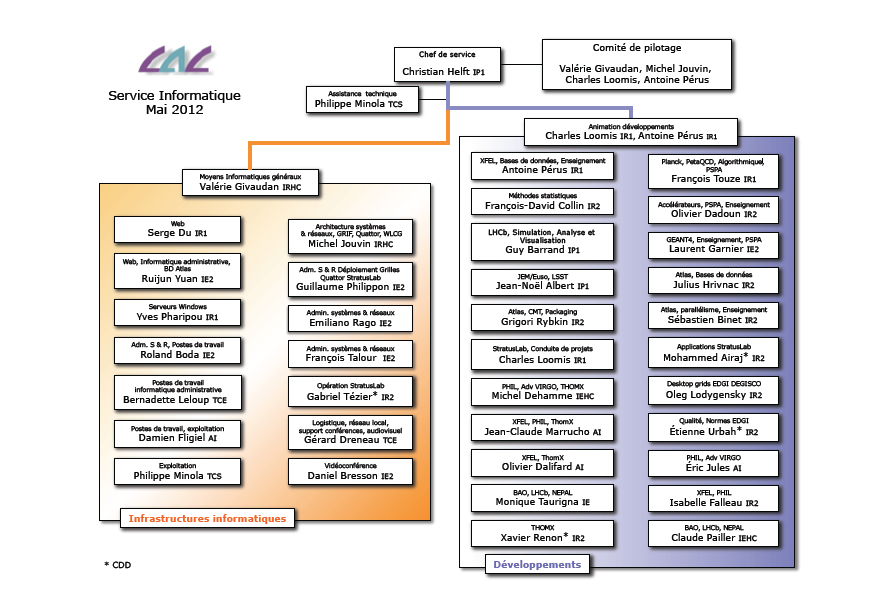
\includegraphics[scale=0.7]{img/si_organigramme}
	\caption{Organigramme du service informatique}
	\label{fig:siorga}
\end{figure}

Le service informatique est responsable de la mise en place, de la maintenance
et du support de tout le système informatique du laboratoire. Il est aussi impliqué dans 
les nombreux développements logiciels pour les expériences auxquelles il participe, avec
des spécialistes de nombreux domaine de l'informatique : base de données, visualisation,
parallélisme, contrôle-commande d'appareillages, calcul numérique... Il s’occupe
également du développement et de l’exploitation de plusieurs logiciels utilisés
par le personnel du laboratoire pour le travail scientifique ou administratif.

L’équipe exploitation s’occupe de toute l’infrastructure informatique du
laboratoire, comprenant la maintenance et l’installation des postes de travail
ou des serveurs demandés par les membres du laboratoire.

Logiciel \emph{GLPI} était utilisé pour la gestion de ticket
par l’équipe exploitation du service informatique du laboratoire. Ainsi, toute
personne qui a le moindre problème avec le parc informatique du laboratoire et
tous les services qu’il comprend ou la moindre suggestion ou demande qui le
concerne peut créer un ticket sur ce système afin de suivre l’évolution de son
problème ou de sa demande.  GLPI possède aussi des fonctionnalités de gestion
de parc qui ne sont pas utilisées au LAL.

Les membres du service ont aussi mise en place un site d'une grille de
calcul (la grille EGI) qui est utilisée par des chercheurs à travers le monde entier pour
effectuer des calculs complexes demandant de grosses ressources. Ce site, GRIF, dispose
ainsi de 8000 cœurs de calculs et d’un stockage de 3.5~pétaoctets de données.
L’objectif est qu’elle soit à terme remplacée par la solution de Cloud \emph{StratusLab}.
Une équipe du LAL est impliquée dans le développement et la maintenance de ce
logiciel, issue d'un projet européen FP7.
Le cloud StratusLab du LAL disposait fin 2012 de
250~cœurs de calculs et 30~téraoctets de stockage et doit être augmenté cette
année à 500~cœurs et 60~téraoctets.Ce cloud estouvert aux utilisateurs de plusieurs
laboratoires, de l'université Paris Sud en particulier. L'idée est de construire une ressource
mutualisée entre tous pour permettre à chacun de profiter de l'ensemble des ressources
quand les autres ne les utilisent pas.

Enfin, certains membres du service donnent des cours aux étudiants de
l’université Paris-Sud, située sur le même campus.

\section{Contexte du stage}
\label{sec:context}

Le stage s’inscrit dans la volonté du service de rénover ses
infrastructures. Il utilise par exemple pour plusieurs services un cluster de
très vieilles machines sous Unix Tru64 dont il aimerait se débarrasser. Un certain
nombre de procédures sont également très vieilles et gagneraient à être
simplifiées, ce qui est le cas pour la gestion des adresses IP du laboratoire.

De plus, même si cela n’a pas influé sur la création du stage par le
laboratoire, le projet de rénovation des laboratoires de \emph{P2IO} a été
annoncé et doit permettre en une modernisation globale des laboratoires situés sur le
campus de l’université Paris-Sud.

Ce vaste projet prévoit par exemple~:

\begin{itemize}
	\item une rénovation et un désamiantage des bâtiments,
	\item une mise aux normes des bâtiments quant à l’obligation d’accès aux
	personnes à mobilité réduite,
	\item la création d’une salle informatique commune aux laboratoires, dans le
	cadre du projet \emph{Virtual Data}, permettant une mutualisation des
	ressources informatiques des laboratoires,
	\item l’amélioration de la répartition des équipes au sein des locaux, ce
	qui implique le déménagement d’un grand nombre de personnes.
\end{itemize}

Pour le service informatique, cela pourrait impliquer le déménagement de l’équipe
vers un autre endroit. A plus court terme (automne 2013), il va s'agir de déménager la salle machine actuelle
vers la salle machine commune \emph{Virtual Data} en cours de construction.\\

Le stage était motivé initialement par la volonté d'automatiser un certain nombre
de procédures très manuelles avec tout les risques d'erreur et d'incohérence inhérents.
Ce besoin initial s'est trouvé renforcé par le départ à la fn 2012 de Damien
\textsc{Fligiel}, qui était chargée du support aux postes utilisateurs sous
Windows et était à ce titre le pincipal responsable de la déclaration manuelle des nouvelles machines
dans le DNS et DHCP.

\newpage

\chapter{Travail effectué}

Le travail effectué au cours de ce stage a été consacré au développement d’un
outil de gestion de l’allocation des adresses IP au laboratoire et à sa mise en
production.

\section{Cahier des charges}

Le cahier des charges a été défini au cours d’une réunion préliminaire avant
le début du stage et au cours de nombreuses réunions courtes au cours du stage
pour le suivi de l’avancement du projet et la précision de certains de ses
aspects.

\subsection{But du logiciel}

Le but du logiciel développé au cours de ce stage est de fournir une solution
de gestion automatique des adresses IP pour le laboratoire. Il doit pour cela
fournir un moyen de manipuler des ressources comme des adresses, des
collections d’adresses et des hôtes et, pour chacune de ces entités, avoir la
possibilité de les créer, modifier ou supprimer ainsi qu’un certain nombre de
données auxiliaires les concernant. En plus d'une interface de base en ligne
de commande, il doit aussi fournir une interface à base de formulaire web
pour permettre à des non spécialistes de faire la configuration réseau d'une
nouvelle machine.

Enfin, une fois que les données sont correctement créées dans le logiciel,
celui-ci doit offrir la possibilité de générer les fichiers de configuration
d’un certain nombre de services réseau tels que le serveur DNS ou le serveur
DHCP.

Un cas d’usage typique correspond à l’insertion d’une nouvelle machine dans le
réseau du laboratoire~: un membre du service informatique remplit les
informations concernant la machine (nom, alias, numéro de série et
d’inventaire, adresse MAC, catégorie de machine, propriétaire\dots) sur un
formulaire Web ou en ligne de commande. Il n’a ensuite qu’a lancer une autre
commande ou cliquer sur un bouton de l’interface Web pour régénérer les
fichiers de configuration et relancer les services réseaux en prenant en
compte les modifications.


\subsection{Existant}

L’infrastructure existante comprend un serveur DNS qui tourne sur un cluster de
machines UNIX ainsi qu’un serveur DHCP.

Le serveur DNS utilise un format de fichier personnalisé pour avoir un format
simple permettant de définir un hôte en une ligne, ainsi que tous ses alias de
nom et ses serveurs de messagerie électronique. Il permet également de séparer
une zone DNS en plusieurs fichiers ce qui n’est pas directement possible avec
l’implémentation DNS utilisée. Un script TCL doit ensuite être lancé par le
biais d’un \emph{Makefile} afin de transformer ce format de fichier
personnalisé vers le format de zone DNS tout en générant les résolutions
inverses des noms et en faisant diverses vérifications, sur l’unicité des noms
par exemple.

Le serveur DHCP utilise quant à lui le format standard qui permet d’inclure des
fichiers, et donc sépare nativement les machines en plusieurs groupes, ce qui
est très utile pour rendre gérable manuellement le grand nombre de machine
(~1500). Les modifications sont effectuées sur le cluster de machines
UNIX et ensuite envoyées au serveur DHCP réel.

Pour les deux services, des vérifications sont effectuées sur les données et,
en cas d’erreur, les modifications ne sont pas appliquées aux serveurs en
production.

\subsection{Cœur du logiciel}
\label{sec:core}

Le logiciel à développer au cours du stage manipule un certain nombre de
notions clés qu’il est important de bien définir~:

\begin{description}
	\item[Pool] correspond directement à la notion réseau de plages d’adresses
	c'est-à-dire une collection d’adresses, la plupart du temps contiguë,
	mais pas obligatoirement. C’est donc parmi un ou plusieurs \emph{Pool}s que
	seront prises les adresses à allouer.
	\item[Host] Identifie de manière unique un hôte nommé sur le réseau et qui
	peut correspondre à une machine physique (ordinateur de bureau, ordinateur
	portable, serveur…), une machine virtuelle (VM) ou bien relevant de cas
	particuliers tels que les machines présentant une interface
	IPMI\footnote{Intelligent Platform Management Interface, une interface qui
	permet l’administration à distance des machines par un système indépendant
	du système d’exploitation de la machine. Le fait que l’interface IPMI soit
	distincte du système de la machine permet de garder la main sur la machine
	même en cas d’erreur grave dans le système d’exploitation et peut continuer
	à fonctionner même si la machine est éteinte. Mais cette indépendance qu’a
	l’interface IPMI du système hôte fait que d’un point de vue du réseau les
	deux seront vues comme deux hôtes différents.}, mais qui
	seront traitées comme des hôtes normaux.
	\item[Address] Adresse qui identifie de manière unique un \emph{Host} sur
	le réseau et regroupée dans des \emph{Pool}s.
\end{description}

Ces différentes notions se retrouveront dans le modèle de donnée adopté.\\

Sachant cela, le but principal du programme final est de mettre en relation les
\emph{Pool}s et les \emph{Host}s grâce aux \emph{Address}.

\subsection{Technologies choisies}

\subsubsection{Langage~: \emph{Python2}}

Python a été choisi, car c’est un langage expressif et compact qui bénéficie
d’une très bonne documentation et d’un bon support de la communauté. Il peut
être interfacé avec de nombreuses autres entités et technologies grâce à un
très grand nombre de modules. C'est un language particulièrement bien adapté
à l'écriture d'application web.

Le choix d’utiliser la version 2 plutôt que la 3 découle du choix d’utiliser le
framework \emph{Django} (voir la section \ref{sec:framework-django}). En effet,
à l’époque du stage, \emph{Django} n’était disponible que pour la version 2 de
Python.

\subsubsection{Framework~: \emph{Django}}
\label{sec:framework-django}

\emph{Django} est un framework Python qui a pour but de faciliter le
développement d’applications Web modernes. Il met ainsi à disposition des
développeurs un grand nombre de modules fournissant toutes les
fonctionnalités nécessaires au développement d’applications Web.

Il fournit par exemple des mécanismes pour~:

\begin{itemize}
	\item générer les pages dynamiquement avec un système de templates très
	complet et intuitif,
	\item un ORM\footnote{\emph{Object-relational mapping}, ici utilisé pour
	manipuler des données de la base de données comme des objets du langage
	Pyton} très puissant qui présente une interface abstraite pouvant
	s’adapter à différent SGBD\footnote{Système de gestion de base de données,
	telle que MySQL, Oracle, PostgreSQL\dots},
	\item gérer plusieurs langues permettant à l’utilisateur de changer de
	langue à la volée à tout moment et, côté développeur, de centraliser tous
	les fichiers de traduction pour faciliter la traduction du logiciel,
	\item fournir une manière souple et avancée d’organiser le contenu du site,
	\item gérer les utilisateurs et le contrôle d’accès à certaines parties du
	site en fonctions des droits de ces utilisateurs, et qui peut être
	interfacé à d’autres systèmes d’authentification tels qu’un annuaire
	\emph{LDAP} qui a, par exemple, été utilisé dans le logiciel développé au
	cours de ce stage,
	\item protéger le site des failles de sécurité les plus courantes.
\end{itemize}
~\\

Il avait été initialement décidé de ne pas utiliser l’ORM de \emph{Django,}
mais plutôt \emph{SQLAlchemy}. Cette décision a été abandonnée rapidement, le
maître de stage considérant que cela entraînerait plus de complexité pour le
développement sans apporter de réel bénéfice.

\subsubsection{Autres technologies}

Le gestionnaire de version \emph{Git} a été utilisé. Il facilite, grâce à
gestion très souple des branches, la possibilité de développer plusieurs
fonctionnalités ou corrections de bug en parallèle et sans difficulté ce qui
est assez avantageux pour un développement \emph{AGILE} où des décisions
peuvent être changées régulièrement ou abandonnées au cours de réunions
régulières.

\emph{Sphinx} a été utilisé comme outil de documentation, car il est simple à
utiliser et s’interface bien avec Python. Il permet par exemple d’écrire la
documentation sur le fonctionnement interne sous forme de commentaire au sein
même du code. \emph{Sphinx} sera ensuite capable de récupérer la structure du
code (les classes, leurs attributs, les fonctions, etc.) ainsi que tous les
commentaires les concernant afin d’en générer une page de documentation bien
structurée.

Le serveur d’intégration \emph{Jenkins} a été utilisé afin d’effectuer une
intégration continue du logiciel. Il possède un très grand nombre de plug-ins
qui permettent de s’interfacer avec une grande variété d’outils et système
différents.

Il a été choisi d’utiliser \emph{NOSE} comme framework de test pour construire
une série de tests unitaires et fonctionnels autour du logiciel développé. Des
plug-ins permettent en plus d’obtenir le taux de couverture du code par les
tests ce qui permet de mieux se rendre compte des parties du code qui pourront
potentiellement poser problème en étant insuffisamment testées. Un autre
plug-in permet de générer un fichier de statistiques standards qui pourra
ensuite être utilisé par le serveur \emph{Jenkins} pour dessiner des graphiques
sur les données des tests.

Enfin, le logiciel \emph{TRAC} a été utilisé comme interface de gestion de
projet, pour avoir une documentation basique et éventuellement un système de
tickets. Il a été choisi, car c’est le système utilisé par tous les projets du
service et il est donc déjà en place. Il permet de plus de s’interfacer
facilement avec plusieurs systèmes de versionnement tels que \emph{Git,}
utilisé pour ce stage, et permet ainsi de suivre les avancées du projet sans
être obligé d’utiliser les méthodes spécifiques fournies par le logiciel de
contrôle de version.\\

\subsection{Interface en ligne de commande}

L’interface en ligne de commande doit pouvoir permettre de contrôler toutes les
opérations du programme depuis une invite de commande en console.\\

Il a été défini dès le début du stage que le logiciel devait disposer d’une
interface en ligne de commande afin de pouvoir interagir avec elle en se
connectant à des serveurs et surtout de pouvoir intégrer le logiciel dans des
scripts pour automatiser des operations.

\subsection{Interface Web}

L’interface Web doit permettre de fournir le moyen d’interagir avec le
logiciel le plus simple et intuitif possible afin que toute personne
du service puisse effectuer les actions principales rapidement et sans avoir
besoin de lire la documentation de l’interface en ligne de commande.

Pour cela, le \emph{framework} \emph{Django} a été pleinement utilisé pour la
réalisation de cette interface, et a grandement aidé pour sa mise en place
grâce à la très grande facilité d’échange d’information entre la base de
données et le système de \emph{templates} qui génère réellement l’interface.

Il était important de pouvoir accéder aux fonctionnalités du logiciel par une
interface REST (Representational State Transfer) qui permet de s’appuyer sur
les méthodes du protocole HTTP \verb+GET+, \verb+POST+, \verb+PUT+ et
\verb+DELETE+ et les nombreux codes d’erreur adaptés à différentes situations.Ceci permet
de contrôler le logiciel depuis un script ou une machine
sans interface graphique, tout en bénéficiant des fonctionnalités avancées
de l'application web, comme l'authentification. Pour renvoyer les données, le format \emph{Json} a
été utilisé, c’est un format simple et suffisamment répandu pour que des
modules d’analyse et de récupération des données soient disponibles pour la
plupart des langages. La gestion des templates de Django permet très simplement
de mutualiser tous les traitements et de spécifier deux formats de sortie très
facilement. Django ne peut pas gérer par défaut les différentes méthodes HTTP,
mais un module permet de remédier à ce problème.

\subsection{Importance de la future maintenabilité}

Dès le début du stage une grande importance a été accordée à la documentation
produite et aux tests du programme dans le but de faciliter la maintenance une
fois le stage terminé. Il a été aussi évoqué la libération du code, sous forme
de paquet python et sa mise à disposition sur le site \emph{Github}.

Il a ainsi été décidé d’utiliser le paquet python \emph{Sphinx} qui permet la
rédaction d’une documentation dans un format simple et lisible avec la
possibilité de générer ensuite la documentation dans de multiples formats
différents (PDF, HTML\dots). Il a été question d’interfacer cette documentation
avec l’outil de gestion de projet utilisé par le laboratoire, \emph{TRAC}. Cet
outil propose en effet un moyen interne de gérer la documentation des projets
sous forme de \emph{Wiki}, c'est-à-dire de pages Web éditables avec une syntaxe
dédiée, mais permet également, grâce à un paquet python spécial, d’accepter le
format \emph{Sphinx}, ce qui serait très utile pour le projet en question.

\newpage

\section{Déroulement du stage}

Le stage s’est déroulé du 3 septembre 2012 au 18 janvier 2013 au sein de
l’équipe exploitation du service et encadré par Antoine \textsc{Pérus},
responsable de l’équipe développement.

\subsection{Familiarisation avec l’environnement}

Une présentation succincte du laboratoire et du service ont tout d’abord eu lieu
ainsi qu’une présentation des principales personnes avec qui le
stagiaire allait interagir. Les diverses tâches administratives ont été
accomplies, avec, par exemple, la création d’un compte sur le système
informatique du laboratoire afin de pouvoir accéder à l’ensemble des services
utiles pour le stage.

Les premiers jours du stage ont été dédiés à l’installation de l’environnement
de travail. La distribution de Linux \emph{Ubuntu} a été installée sur un
ordinateur de bureau par le stagiaire. Ce choix de s’orienter vers un
environnement UNIX a été fait selon les préférences du stagiaire et par ce que
l’environnement de développement sous Python est bien intégré à ce type de
système. Les outils nécessaires au développement ont ensuite été installés~:

\begin{itemize}
	\item \emph{Git} pour versionner les changements du logiciel développé,
	\item \emph{Python2}, \emph{Django} et les paquets nécessaires au
	développement,
	\item \emph{Sphinx} pour la génération de la documentation,
	\item \emph{Nose} et \emph{Pylint} pour la vérification de programme et la
	détection de bugs,
	\item \emph{Vim}, éditeur utilisé pour l’écriture du code
\end{itemize}
~\\

Une réunion avait été organisée avant le début du stage afin de régler
les différents détails du projet. C’est le compte rendu de cette réunion qui
servira de cahier des charges initial pour le démarrage du projet. Ces points
ont été éclaircis par la suite au travers de questions posées à différents
membres de l’équipe, responsables des différentes parties impactées par le
projet.\\

Le stagiaire s’est ensuite familiarisé avec le langage Python qu’il avait un
peu pratiqué, mais devait revoir plus en détail ainsi que toutes les
caractéristiques du framework Django. Le meilleur endroit pour trouver des
documentations sur ces deux composants est leurs sites officiels respectifs qui
intègrent une documentation extrêmement complète et intuitive.

\subsection{Développement du logiciel}

La conception du logiciel même a alors pu commencer, avec, en priorité,
l’architecture du cœur du logiciel. Comme expliqué en section \ref{sec:core}
page \pageref{sec:core}, il a été prévu que le logiciel repose sur trois
classes principales~:

\begin{itemize}
	\item \emph{Pool} qui représente une collection d’adresses,
	\item \emph{Host} qui représente une machine physique ou virtuelle,
	\item \emph{Address} qui représente une adresse allouée.
\end{itemize}

L’idée a donc été, dans un premier temps, d’avoir différentes classes
représentant une plage d’adresse, en fournissant, de base, une classe pour les
IPv4, une classe pour les IPv6 et une classe pour des adresses arbitraires. Ces
classes sont ensuite encapsulées indifféremment dans la classe \emph{Pool} qui
s’occupe de stocker des données supplémentaires et garde la trace des adresses
qui sont utilisées ou non dans la collection d’adresse.

Ces trois classes ont donc tout d’abord été créées avec une interface
permettant de parcourir la collection complète d’adresses, d’obtenir une
adresse, de récupérer sa taille, etc. C’est également ces classes qui
s’occupent d’analyser le format pour exprimer les adresses IP sous forme
d’adresse de réseau et masque du type \verb+127.13.37.42/24+, qui fonctionnent
en IPv4 et IPv6. Ces trois classes ont toutes été documentées et toutes leurs
fonctions ont été testées. Cela a permis de tester tout le système de
documentation et de tests unitaires et fonctionnels ont pu être mis en place.

\begin{center}
\begin{figure}[hbt]
	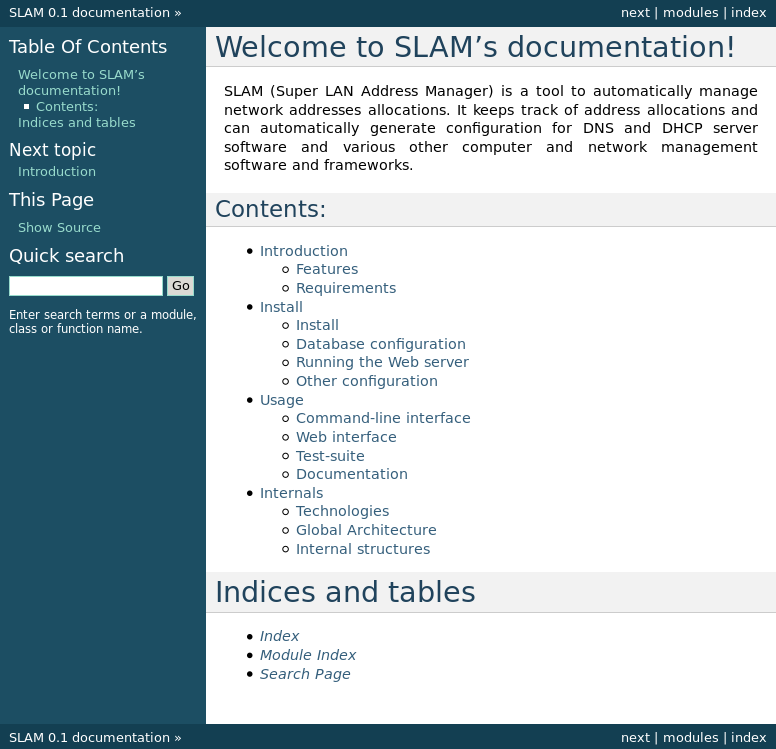
\includegraphics[scale=0.45]{img/doc.png}
	\caption{Documentation de SLAM}
	\label{fig:doc}
\end{figure}
\end{center}

L’outil de documentation \emph{Sphinx} a donc été installé et configuré. Il
suffit ensuite de rédiger la documentation sous forme d’une arborescence de
documents écrits dans un format spécifique (\emph{reStructuredText}).
La commande d’initialisation permet de créer un fichier \emph{Makefile} qui
pourra être utilisé pour générer différents formats de fichiers (HTML,
PDF\dots) à partir du format source \emph{reStructuredText}. Le résultat final
en HTML est présenté en figure \ref{fig:doc}.

\emph{Nose}, utilisé pour la réalisation de tests, requiert que des tests
soient écrits en Python sous forme de fonctions. Il exécutera ensuite toutes
les fonctions dont le nom est conforme à une certaine norme séquentiellement.
Il est donc possible dans chacune des fonctions de tests d’exécuter tout le
code nécessaire aux tests sans aucune restriction, ce qui permet donc de
réellement tester tous les aspects du programme développé sans problème. S’il
est nécessaire d’exécuter du code avant ou après un ensemble de fonctions de
tests, \emph{Nose} permet de déclarer des fonctions d’initialisation ou clôture
des tests. Une fois ces fonctions déclarées, il suffit de remplir un fichier
de configuration pour \emph{Nose} et de lancer le script de \emph{Nose} pour
exécuter l’ensemble des tests et afficher un rapport détaillé incluant les
messages générés par les tests qui ont échoué. Ces fonctionnalités permettent
donc d’écrire des tests unitaires pour tester le bon fonctionnement de chaque
fonction du programme en vérifiant les bonnes valeurs pour différentes valeurs
d’arguments, mais aussi des tests fonctionnels permettant de vérifier le bon
fonctionnement de l’interface que le programme expose aux utilisateurs ou à
d’autres développeurs à travers une éventuelle interface de programmation.

Une interface basique sera aussi développée et constituera l’embryon de
l’interface en ligne de commande, en permettant de créer des pools et de
récupérer un certain nombre d’adresses choisies linéairement. Cela a permis la
découverte du module \emph{Argparse} de Python, permettant ainsi une
configuration sommaire du logiciel grâce aux arguments de la ligne de commande.
L’écriture de tests pour cette interface a permis la réelle constitution de
tests fonctionnels pour l’application.\\

En partant sur cette base fonctionnelle et testée, l’ORM de Django a dû être
intégré afin de pouvoir stocker des données de manière persistante dans une
base de données supportée par Django. Cet ORM est constitué de tout un
sous-module de Django qui se charge de faire la transition entre le modèle de
classes et de types internes à Python vers le système de tables et de types
d’une des bases de données supportées par Django. Côté développeur, il suffit
de déclarer des classes héritant d’une classe \verb+Model+ de Django avec des
attributs qui correspondront aux attributs des tables dans le modèle des bases
de données et Django s’occupera de faire la correspondance entre les deux. Une
fois ces classes déclarées, il suffit d’instancier un objet pour créer un
nouvel enregistrement dans la base de données, des méthodes sont ensuite
héritées pour supprimer cet enregistrement ou sauvegarder les modifications.
Grâce à cette abstraction, Django peut s’adapter à plusieurs bases de données
différentes sans que le développeur n’ait besoin de changer son code ou son
modèle de données. Django est ainsi fourni de base avec le support de MySQL,
SQLite, PostgreSQL et Oracle, seuls l’adresse du serveur et les identifiants
sont à changer. Ainsi une base SQLite aura été utilisée pendant le
développement du logiciel et une base de données MySQL pour le déploiement en
production.

Une contrainte additionnelle est de devoir utiliser les types spécifiques de
Django afin qu’il puisse les convertir correctement vers les types des bases de
données. Il faut donc prévoir des méthodes pour sérialiser les classes
complexes telles que les collections d’adresses IPv4 ou IPv6 vers un type
chaîne de caractère par exemple avant la sauvegarde de l’objet, et la
restauration correcte de l’objet à partir d’une chaîne de caractères. Mais la
conversion des classes existantes et l’ajout n’a pas engendré de grande
difficulté.

Il a ensuite fallu adapter toute la suite de tests et l’interface en mode
ligne existante pour tester et fournir un accès aux nouvelles méthodes
permettant de créer, lister, modifier et supprimer un Pool existant ainsi que
de pouvoir récupérer une adresse disponible dans un Pool existant et de garder
trace des adresses utilisées. L’interface en mode ligne a donc été refaite
quasiment entièrement et tous les tests associés aussi.

C’est aussi à ce moment que les classes Host et Address ont commencé à être
utilisées et étendues. Des attributs d’information ont été ajoutés à ces deux
classes, comme leur donner un nom et une adresse MAC, qui est l’adresse
physique d’une carte réseau d’une machine. Avec pour chacune de ces classes la
possibilité d’ajouter, modifier ou voir les informations des objets de ce type
dans la base de données.

L’analyseur statique \emph{Pylint} a d’ailleurs été ajouté à la suite de tests,
en permettant de détecter, sans interpréter le code, des erreurs ou ambiguïtés
potentielles du code et les signaler. Il est possible de configurer un grand
nombre de variables dans les erreurs qu’il recherche et de fixer des limites
comme le nombre de lignes par fonction, le nombre de branches conditionnelles
imbriquées, etc. selon les préférences du développeur. Un certain nombre
d’erreurs ont ainsi pu être corrigées grâce à cet outil, en prévenant des bugs
éventuels avant même qu’ils ne se manifestent.\\

Un serveur d’intégration continue \emph{Jenkins} a également été mis en place.
Ce serveur codé en Java a pour rôle de sonder le dépôt \emph{Git} afin de
détecter les changements et, dans notre cas, de lancer la suite de tests ainsi
que l’analyseur statique sur le programme afin d’envoyer un rapport au
stagiaire si jamais un problème survient. Par la suite, ce serveur s’occupera
également de construire la documentation au format HTML et de la copier sur un
serveur HTTP pour avoir une documentation à jour accessible. Pour installer ce
serveur, une machine virtuelle a été préparée sur le système de gestion de
Cloud développé au laboratoire~: \emph{StratusLab}.

StratusLab permet de mettre en commun des ressources physiques pour former un
Cloud, sur lequel les utilisateurs peuvent ensuite créer un nombre quelconque
de machines virtuelles aux caractéristiques variables et personnalisables, dans
la limite des ressources disponibles. Le principe est donc que plusieurs
services ou laboratoires fournissent des moyens physiques pour l’agrandissement
du Cloud, pour pouvoir offrir à leur utilisateur un accès quand ils le
souhaitent. Les utilisateurs enregistrés ont juste à choisir les
caractéristiques de leur machine virtuelle à créer et à choisir dans le
\emph{Marketplace} une image de système d’exploitation pré configuré contenant
éventuellement des paquets préinstallés. Pour le stage, une image de CentOS~6
aura par exemple été choisie avec un serveur Jenkins préinstallé ainsi que ses
dépendances. Il aura ensuite été nécessaire d’installer toutes les dépendances
demandées par le logiciel développé, c'est-à-dire Python, Django et tous les
modules annexes ainsi que Git pour la récupération des sources.

La configuration de \emph{Jenkins} est ensuite très simple et se fait par une
interface Web, quelques paramètres doivent être donnés au moment de la création
du projet sur l’interface ainsi qu’au module Git permettant de surveiller les
changements sur le dépôt de sources. Il existe des moyens de lancer des tests
pour des applications Java directement depuis Jenkins, mais cela ne correspond
pas à ce qui est recherché. L’option utilisée est l’exécution d’un script shell
qui va lancer toute la suite de tests. Un script a donc été écrit spécialement
dans ce but, qui lance la suite de tests, l’analyseur statique \emph{Pylint} et
construit la documentation.

Un dernier point intéressant est que la distribution CentOS utilisée sur la
machine virtuelle dans sa version 6 ne proposait le paquet Python que dans sa
version 2.6 alors que le développement était réalisé avec une version 2.7 qui
est la version la plus à jour. Or il faut savoir qu’un certain nombre de
serveurs de production ne disposent que de la version 2.6, il a donc été décidé
de fournir le logiciel développé pour les versions 2.6 et 2.7 de Python afin de
viser un maximum de machines. La machine virtuelle a donc été également utile
pour tester régulièrement la bonne compatibilité du logiciel avec Python~2.6.
Plusieurs modifications ont dû être effectuées suite à cette décision puisque
le code utilisait plusieurs fonctionnalités qui ne sont apparues que dans la
version 2.7 de Python. Il ne s’agissait que de changements mineurs portant
sur une différence de syntaxe entre les deux versions concernant la création de
Sets pour laquelle la version 2.6 requiert un appel explicite à la fonction
\verb+set()+ et pour l’utilisation de la fonction \verb+format+ permettant le
formatage avancé de chaînes de caractères pour laquelle la version 2.6 exige
l’index explicite des arguments contrairement à la version 2.7.\\

Une meilleure gestion des erreurs a ensuite été développée par le stagiaire, se
traduisant par une meilleure détection des erreurs de saisie dans les entrées
de l’utilisateur et en prévoyant les problèmes internes pouvant survenir au
cours des traitements effectués. Des tests ont été ajoutés pour tester le fait
que les différentes erreurs potentielles sont bien gérées par le logiciel grâce
à une fonction de \emph{Nose} permettant de tester les cas d’erreur très
simplement.  La documentation a aussi été complétée pour documenter les
nouvelles options de l’interface en ligne de commande. Par ailleurs, de
nouvelles pages ont été créées pour expliquer le fonctionnement interne de SLAM
et certains choix d’architecture ou des détails subtils, afin d’aider un futur
mainteneur, à mieux comprendre l’architecture et le code du projet et à le
guider.

La notion de propriété a été ajoutée aux pools et aux hôtes, c'est-à-dire la
possibilité d’attacher n’importe quelle information arbitraire à l’un ou
l’autre en précisant le nom de la propriété et sa valeur. Cela permet
d’étendre le nombre de champs de ces deux objets sans contrainte particulière.
On peut par exemple imaginer sauvegarder l’adresse email du propriétaire d’une
machine avec ce système ou indiquer le numéro de bureau d’une machine, etc.
\label{sec:property}

C’est à partir de ce moment que le stagiaire a expérimenté le \emph{Test-driven
development}, du développement piloté par tests, c'est-à-dire à écrire les
tests pour une fonctionnalité ou une fonction avant d’écrire le code même
fournissant cette fonctionnalité. Cela permet d’obtenir des tests de meilleure
qualité puisqu’ils testent réellement le comportement attendu d’une fonction
en fonction des différentes valeurs de ses paramètres, au lieu de n’être écrit
qu’en fonction du code de la fonction et avec pour simple objectif que le test
associé réussisse avec la forme actuelle de la fonction comme c’est le risque
si le test est écrit a posteriori.\\

Une partie importante du projet a été entamée à ce moment et concerne la
génération des fichiers de configuration. Un ensemble de classes de
configuration a ainsi été créé pour s’occuper du format DHCP, DNS et Quattor.
Sur le même modèle que la classe Pool, une classe générique \emph{Config} a été
créée de laquelle ces différentes classes pour les différents formats
héritent en fournissant plusieurs autres fonctionnalités. C’est ainsi cette
classe qui permet de faire la différence entre la création d’un nouveau fichier
de configuration et la mise à jour d’un fichier existant, où seule la partie
réservée à notre outil, SLAM, sera mise à jour, le reste étant conservé. Elle
offre également la possibilité d’inclure un fichier d’en-tête et un de
pied de page afin d’ajouter des informations complémentaires non gérées par
notre outil. Ces fonctionnalités sont paramétrables pour chaque générateur~: la
configuration du DNS va par exemple vérifier si un enregistrement SOA existe
dans le fichier actuel pour les en-têtes, alors le champ \emph{serial} associé
sera mis à jour selon les règles conseillées dans la RFC~1912 présentant les
bonnes pratiques pour la gestion d’une zone DNS.

Une grande partie des tests de cette partie a été réalisée avant son
développement réel, mais a été complétée par certains cas capricieux rencontrés
au cours du développement. La documentation était, comme pour tout le reste du
code, écrite directement sous forme de commentaires au milieu du code et
récupérée par un module Python. Il est important de noter que ces
configurations ne sont pour l’instant pas sauvegardées dans la base de données
et qu’il est donc nécessaire de préciser toutes les options utiles à la
génération des fichiers comme le format de fichier à générer, le chemin du
fichier et les éventuels fichiers d’en-tête ou de pied de page.\\

Environ un mois après le début du stage, au cours de la réunion d’exploitation
hebdomadaire, l’interface en ligne de commande de SLAM, la solution développée,
a été présentée à l’équipe d’exploitation et plusieurs commentaires et
critiques ont pu être recueillis. L’interface a globalement été jugée peu
intuitive ou peu compréhensible, le fait d’être obligé de préciser toutes les
informations à la création ou mise à jour des fichiers de configuration a été
jugé rédhibitoire et il a été suggéré de changer le nom du script principal qui
était \verb+slam_cli+ vers \verb+slam_adm+ ou, plus simplement, \verb+slam+.

À peu près tous les problèmes relevés ont été réglés dans la semaine. La
configuration de la génération des fichiers de sortie est donc devenu une
information persistante stockée dans la base de données. Ces informations ont
donc été regroupées dans une classe \emph{Generator}, désignée uniquement par
un nom et ayant pour but de stocker les informations utiles aux différentes
classes de configuration. Cette nouvelle classe est donc désignée par un nom et
stocke les chemins du fichier à générer et des fichiers d’en-tête et de pied de
page. Le type de fichier à générer et des éventuels Pool associés auxquels
limiter la génération. Le problème est que ce nouvel ajout d’information a
engendré une nouvelle complexité à l’interface, qui était déjà compliquée
d’après les commentaires recueillis. L’interface a donc été légèrement
simplifiée et de très nombreux exemples ont été ajoutés dans la documentation
en illustrant un grand nombre de cas pratiques utiles pour toutes les
utilisations possibles de SLAM. Cette grosse modification de l’interface a
demandé une réécriture d’un grand nombre de tests.

Dans ce même but de simplifier l’interface, la notion de catégories d’hôte a
été ajoutée, une catégorie du type \emph{PC}, \emph{Mac}, \emph{Server} ou
\emph{VM} pouvant être ajoutée à un hôte et les Pools pouvant contenir une
liste de catégories pour indiquer la liste des différents types de machines
qu’ils acceptent. Le but de cette opération est qu’un utilisateur ait
simplement à indiquer les informations d’une machine, en précisant de quelle
catégorie de machine il s’agit pour que le logiciel sélectionne automatiquement
un pool dans lequel allouer une adresse contrairement à ce qui existait
auparavant qui obligeait l’utilisateur à préciser le nom du Pool dans lequel
allouer l’adresse, ce qui n’était pas forcément le plus intuitif.\\

Après une réunion de suivi du projet avec le maître de stage et plusieurs
personnes du service exploitation, il a été décidé d’attacher de l’importance à
la phase de migration de l’ancien système vers le logiciel SLAM, développé
pendant ce stage. Le système envisagé initialement a été, pour chaque
régénération de la configuration avec SLAM, de rechercher dans les fichiers de
configuration existants si le nom de l’hôte, son adresse MAC ou son adresse IP
n’existait pas et si c’était le cas de générer un message d’erreur explicite à
l’utilisateur comportant le fichier existant et la ligne à laquelle le conflit
a été détecté et d’omettre la ligne de configuration.\\

Le développement de l’interface Web a alors commencé, avec, dès le début, la
gestion en parallèle de l’interface Web standard et de l’interface REST.
L’interface complète a dans un premier temps été réalisée pour la gestion des
pools, des hôtes et des adresses, avec la possibilité de les créer, modifier,
de voir toutes les informations les concernant et de les supprimer (la
suppression d’une adresse équivalent à sa désallocation). Le respect de
l’interface implique que toutes les URL désignent des objets particuliers et
les quatre méthodes HTTP utilisées représentent les différentes actions
réalisables sur ces objets. Des exemples de requêtes sont~:

\begin{itemize}
	\item \verb+GET /host/+ récupère la liste des hôtes de la base de données,
	\item \verb+GET /host/pc-test+ affiche les informations sur l’hôte
	\emph{pc-test},
	\item \verb+POST /host+ crée un nouvel hôte dans la base de données avec
	les informations fournies,
	\item \verb+PUT /pool/server-pool+ modifie le Pool \emph{server-pool} avec
	les informations fournies dans la requête,
	\item \verb+DELETE /host/pc-test+ supprime l’hôte \emph{pc-test},
	\item \verb+DELETE /address/192.168.0.42+ désalloue cette adresse, mais
	conserve l’hôte à laquelle elle était attribuée.
\end{itemize}

Plusieurs difficultés ont dû être résolues pour le bon fonctionnement de cette
interface. Il faut savoir que le standard HTML n’autorise pas la création de
formulaires avec d’autres méthodes HTTP que \verb+GET+ ou \verb+POST+, cela
avait été ajouté à la norme HTML5 en cours de développement, mais a finalement
été retiré.  Il a donc fallu trouver un moyen de contourner ce problème.
Heureusement un module de Django, de type \emph{middleware} a été spécialement
réalisé dans ce but et il est distribué librement. Son rôle est de modifier les
requêtes avant qu’elles ne soient traitées par Django et de modifier les
réponses une fois qu’elles ont fini d’être traitées par Django. Il va donc
transformer tous les formulaires HTML avec des méthodes \verb+PUT+ ou
\verb+DELETE+ et les remplacer par la méthode \verb+POST+, accompagnée d’un
champ caché qu’il pourra reconnaître, et donc, lorsque le formulaire est rempli
par l’utilisateur, il détecte ce champ et remplace la requête \verb+POST+ par
une requête \verb+PUT+ ou \verb+DELETE+ tel que prévu initialement.

Une autre difficulté a été la mauvaise gestion par Django des requêtes en
\verb+PUT+ et \verb+DELETE+ et plus particulièrement la récupération des
données de la requête qui est impossible, car Django n’a prévu de
fonctionner qu’avec les méthodes \verb+GET+ et \verb+POST+, heureusement le
problème est connu et le contournement n’est pas difficile, mais peu élégant
puisqu’il exige de récupérer les données brutes, avant les traitements de
Django pour récupérer les informations intéressantes.

La dernière difficulté rencontrée a été pour écrire les tests de l’interface
Web. Des plug-ins pouvant potentiellement aider ont été étudiés, mais ils
obligeaient toujours à analyser le résultat HTML pour vérifier si la page
générée est correcte. Il a donc été décidé, en accord avec le maître de stage,
de ne tester que l’interface REST avec sortie en \emph{Json}, en sachant que
les traitements sont les mêmes et que seul le format de sortie change grâce au
système de templates de Django. Les tests ont donc été écrits pour cette
interface en couvrant tout ce qui avait été fait sur l’interface Web.\\

La traduction de toute l’interface Web a ensuite été faite. Tous les messages
du logiciel étaient en anglais, de même que la documentation, et la décision a
été prise en réunion de suivi de l’avancée du projet de traduire uniquement
l’interface Web et d’avoir une documentation utilisateur spécifique au
laboratoire en français.

Django fournit tout un mécanisme de traduction très bien intégré. Il suffit
ainsi d’encapsuler toutes les chaînes de caractères à traduire dans des balises
ou des fonctions spéciales et d’exécuter une commande pour que Django récupère
toutes ces chaînes de caractère dans un fichier particulier où le développeur
ou une autre personne, qui n’ont pas forcément de connaissances en
programmation, peuvent écrire la traduction. À partir de ce fichier, Django va
gérer tout seul l’internationalisation des pages et il suffit de proposer une
page à l’utilisateur lui permettant de changer sa langue, ce qu’il peut faire à
n’importe quel moment et toute l’interface sera traduite à la volée sans
problème.

Par ailleurs, un mécanisme est de plus prévu pour des phrases où l’ordre des
mots n’est pas le même suivant les langues grâce à l’utilisation de variables,
comme montré sur cet exemple~:

\begin{lstlisting}
#: views.py:143
#, python-format
msgid "Created pool %(pool)s"
msgstr "Pool %(pool)s cree"
\end{lstlisting}

Une fois toutes ces fonctionnalités ajoutées, le travail s’est porté sur le
renforcement global de l’interface Web en ajoutant, tout d’abord, plus
d’informations sur les pages, en créant beaucoup plus de liens entre les pages
pour pouvoir rapidement accéder aux informations sur un objet avec un simple
clic et, enfin, en ajoutant une meilleure gestion des erreurs avec des
messages explicites et traduits.

La notion de générateurs par défaut a également été créée, les générateurs
étant les instances qui sauvegardent toutes les informations nécessaires à la
génération d’un fichier de configuration (le chemin du fichier résultat, les
pools à générer\dots). Il est possible de définir un ou plusieurs générateurs
par défaut, et ainsi, au moment de lancer la commande pour la génération d’un
fichier de configuration, si aucune option n’est fournie (le nom d’un
générateur, le fichier de sortie, le format à générer\dots), alors l’ensemble
des générateurs par défaut est exécuté. Cela permet de simplifier beaucoup la
génération des fichiers, puisque seule la personne qui connaît les détails du
fonctionnement des serveurs DNS et DHCP par exemple doit configurer toutes ces
options, les autres utilisateurs ne font qu’ajouter ou modifier des hôtes et
n’ont plus à connaître toutes ces spécificités.\\

Après un peu plus de deux mois de stage, la responsable de l’équipe
exploitation, Valérie \textsc{Givaudan}, a voulu que le stagiaire s’occupe de
la gestion de toutes les nouvelles demandes d’adresses IP à venir et des
éventuelles modifications sur ces données. Un rapide apprentissage a donc été
organisé auprès de Damien \textsc{Fligiel}, qui s’occupait, en partie, de cette
tâche et dont le départ du service était proche.

La procédure standard pour ajouter une nouvelle machine est donc la suivante~:

\begin{itemize}
	\item Récupérer une adresse IP libre en sollicitant Philippe
	\textsc{Minola}, assistant technique du service, qui tient manuellement à
	jour une liste des adresses récupérables,
	\item se connecter au cluster Tru64, un cluster UNIX,
	\item ajouter le nom de la nouvelle machine et l’adresse IP associée dans
	les fichiers de configuration du DNS organisés par type de machine,
	\item régénérer la configuration du serveur DNS et relancer le serveur DNS
	à l’aide d’un Makefile fourni,
	\item insérer le nom de la machine et son adresse MAC dans un des fichiers
	de configuration du serveur, eux aussi organisés par type de machine,
	\item lancer un script qui va envoyer les fichiers de configuration du DHCP
	sur un autre serveur et relancer le serveur DHCP qui y tourne.
\end{itemize}
~\\

Il est important de noter que les plages d’adresses utilisées pour les postes
utilisateurs sont toutes utilisées ou l’ont été à un moment, donc la seule
manière pour trouver une adresse libre est de récupérer celles des anciennes
machines qui ont été déclarées comme inutilisées. Mais peu de gens signalent
spontanément qu’une adresse n’est plus utilisée ce qui oblige le service à
appeler les autres services et utilisateurs pour leur demander où ils en sont
dans leur utilisation des adresses et à tenir une liste des ces adresses
réutilisables.\\

À la suite de ce court apprentissage, un compte a été créé pour le stagiaire
sur le logiciel GLPI qui permet à l’équipe exploitation de gérer les tickets
des utilisateurs concernant un problème, une requête ou une tâche à suivre
concernant le système d’information, le logiciel permettant de laisser une
série de messages pour décrire l’évolution de la demande à traiter, une
priorité et un état afin de pouvoir marquer une tâche comme effectuée,
c’est-à-dire fermer le ticket en question. Le but étant que ce soit le
stagiaire qui s’occupe dorénavant de l’allocation des adresses pour réellement
expérimenter toutes les difficultés qui peuvent se poser et quelles choses
peuvent être simplifiées pour cette procédure. Le but est également d’assumer
cette responsabilité pendant la phase de migration durant laquelle la méthode
risque de changer beaucoup.

\begin{figure}[hbt]
	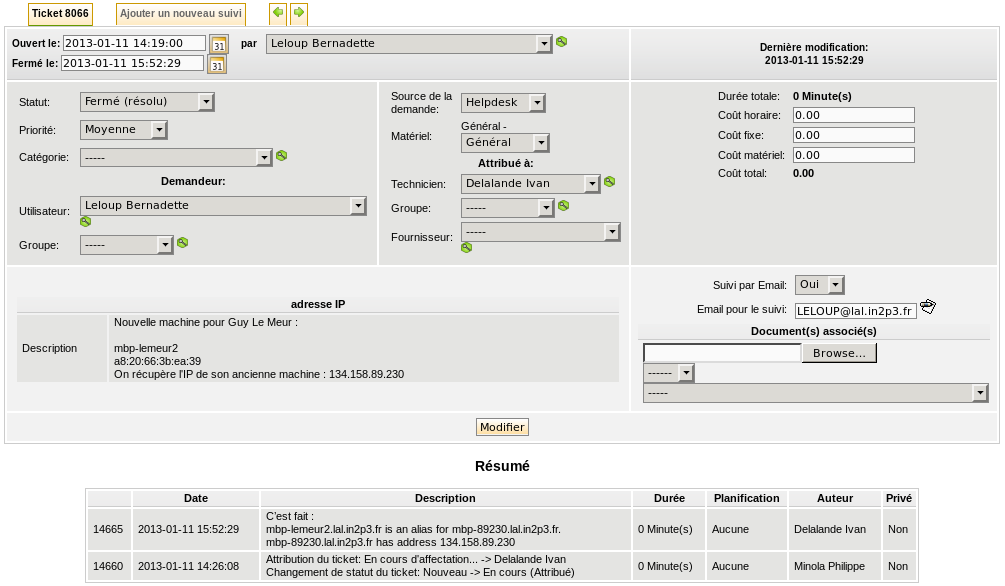
\includegraphics[scale=0.45]{img/glpi2.png}
	\caption{Exemple de ticket GLPI.}
	\label{fig:glpi2}
\end{figure}

Un exemple de ticket est présenté en figure \ref{fig:glpi2}.\\

Une nouvelle réunion de suivi du projet a été organisée et un certain nombre de
questions importantes ont été traitées et résolues à cette occasion. La
première décision prise a été d’ajouter un module de journalisation des
actions effectuées dans la base de données, pour avoir une trace de toutes les
modifications récentes en cas de problème. La question de l’authentification a
été abordée et la solution d’interfacer SLAM avec la base de données
d’utilisateurs déjà enregistrés dans l’annuaire \emph{Active Directory} utilisé
pour la plupart des services du laboratoire a été préférée au fait d’utiliser
une méthode propre à SLAM, nécessitant un développement supplémentaire et
obligeant les utilisateurs à se réenregistrer. Enfin, il a été décidé de
déployer l’interface en ligne de commande sur un serveur la semaine suivante et
de commencer à utiliser ce logiciel pour toutes les nouvelles allocations, tout
en conservant, en parallèle, les fichiers de configuration existants en
attendant la migration totale de la base de données.  Pour prévoir ce
déploiement, une base de données MySQL a été créée pour les besoins spécifiques
de SLAM.

Juste avant le déploiement du logiciel, le système de journalisation a été
développé. Le module de journalisation de Python était déjà utilisé pour
afficher différents messages à l’utilisateur. Il a donc suffi d’ajouter un
collecteur de messages au module de journalisation, tel que documenté afin que
ces différents messages soient également sauvegardés dans la base de données
avec le nom d’utilisateur du logiciel et la date et l’heure où l’action a été
réalisée. Le fait d’utiliser ce même module de Python a permis d’éviter d’avoir
à réécrire tous les messages avec un nouveau système pour chaque action
modifiant la base de données et cela aurait créé du code redondant avec le
système actuel.\\

\subsection{Déploiement}

Le déploiement a démarré, avec une première tentative sur le cluster Tru64. Il
s’agit d’un cluster de machines Alpha sur une variante d’UNIX SystemV développée
par HP et maintenant obsolète et non maintenu. 
Malgré cela, ce cluster, en cours de migration, est encore utilisé pour toutes les opérations de modification
ou d’ajout d’adresses IP dans les DNS et DHCP, ce qui a motivé le stagiaire
pour déployer le logiciel dessus. La version de Python installée sur le
système n’était malheureusement pas à jour, il s’agissait d’une version 2.4
alors que SLAM réclame au moins une version 2.6. La pratique usuelle dans ce
genre de cas est de fabriquer un \emph{virtualenv} avec le module python
éponyme permettant d’avoir une version de Python différente ainsi qu’un
ensemble de modules Python dans un environnement contrôlé et isolé du reste du
système. Cependant, malgré le fait que la compilation de la dernière version de
Python (2.7.3) ait réussi sur ce système, la constitution de l’environnement
virtuel a échoué pour une raison visiblement connue par les développeurs, mais
à laquelle aucune solution n’existe.

Cette solution a donc été abandonnée et il a été évoqué la création d’une
machine virtuelle dédiée aux outils d’administration du réseau et sur laquelle
SLAM aurait sa place. En attendant sa création, une solution de secours a été
proposée par Guillaume \textsc{Philippon} qui est le déploiement de SLAM sur
le serveur hébergeant le logiciel TRAC qui s’occupe de la gestion de tous les
projets du service. Le même problème est cependant survenu, à savoir que la
version de Python installée sur ce serveur était également la 2.4. Mais la
création d’un nouvel environnement virtuel a, cette fois, réussi. L’ensemble
des modules nécessaires à SLAM a donc pu être installé sans problème dans cet
environnement Python dédié.

Le seul problème de cet environnement dédié est qu’il est nécessaire de
modifier sa variable d’environnement \verb+$PATH+ pour pouvoir l’utiliser. Un
script a donc été écrit et placé dans la variable \verb+$PATH+ par défaut du
compte \verb+root+ afin de pouvoir lancer l’interface en ligne de commande par
la simple utilisation de la commande \verb+slam+ sans rien avoir à configurer
en plus, dès la connexion à la machine. Un autre script a de plus été écrit
pour régénérer la configuration et relancer les serveurs DNS et DHCP sur des
machines distantes. Ce script réalise les étapes suivantes et est accessible
avec la commande \verb+slam_reload+~:
\label{sec:slam_reload}

\begin{itemize}
	\item régénération des fichiers de configuration à partir de la base SLAM,
	\item détection du serveur du cluster sur lequel est lancé le serveur DNS
	(il est en effet lancé sur l’une des deux machines du cluster),
	\item régénération des fichiers finaux du DNS avec le Makefile fourni,
	\item redémarrage du serveur DNS,
	\item exécution d’un script sur ce même serveur pour envoyer les fichiers
	de configuration DHCP sur le serveur DHCP placé sur un autre serveur et de
	redémarrer ce serveur DHCP.
\end{itemize}
~\\

En parallèle, le développement du logiciel a continué avec quelques corrections
de bugs découverts au cours du déploiement, mais aussi
l’amélioration constante de l’interface en mode ligne pour simplifier son
utilisation dans la plupart des cas d’utilisation. La sélection automatique du
pool où récupérer une adresse libre a été améliorée pour prendre en compte le
cas où une adresse particulière est spécifiée à la création d’un hôte. Certains
problèmes arrivaient également lors de cette sélection automatique dans
certains cas, mais cela a été corrigé.

Un ajout important a été la prise en charge des alias. En effet, certaines
machines peuvent avoir un alias qui est simplement un nom qui va les désigner
de manière alternative. Ainsi une machine, en plus de son nom peut disposer
d’un ou plusieurs alias. Une classe a donc été ajoutée et représente un alias,
avec son nom, son type (qui va changer la manière dont l’alias est géré par le
générateur de configuration DNS) et une relation vers l’hôte sur lequel cet
alias pointe. Cette relation était tout d’abord de type \emph{ManyToMany},
c'est-à-dire qu’un hôte peut posséder plusieurs alias, mais également qu’un
même alias puisse pointer vers plusieurs hôtes différents. Mais cette dernière
possibilité a été discutée et finalement jugée inutile, donc la relation a été
changée vers une simple clé étrangère permettant uniquement à un hôte de
posséder plusieurs alias, mais pas l’inverse. Cette notion d’alias est ensuite
gérée par le générateur de fichiers DNS qui va générer des enregistrements
\verb+CNAME+ ou des enregistrements d’adresse (\verb+A+ ou \verb+AAAA+ pour le
cas d’IP) selon le type d’alias, même si cette distinction n’est au final pas
utilisée.\\

Pour permettre la migration des données actuelles, deux scripts de migration
ont été écrits, dans le langage de script shell, le premier pour convertir
toutes les données actuelles du DNS en commandes équivalentes pour créer des
hôtes avec le logiciel SLAM et en leur affectant leurs anciennes adresses IP.
Le second utilise les données du DHCP pour modifier ces hôtes et leur attribuer
leurs adresses MAC. Ces deux scripts produisent chacun un nouveau script qui
est composé d’autant de commandes SLAM qu’il y a d’hôtes et qu’il faut alors
exécuter pour importer réellement les anciennes données dans la base SLAM.

Exemple de ligne de configuration DNS pour l’hôte \verb+pc-34125+ avec pour
alias \verb+pc-ivan+~:
\begin{lstlisting}
127.0.34.125	pc-34125	pc-ivan
\end{lstlisting}

Équivalent généré par le script de migration du DNS avec une commande SLAM~:
\begin{lstlisting}
./slam_cli.py --action create --host pc-34125 --alias pc-ivan --category pc --address 127.0.34.125
\end{lstlisting}

Ces scripts ont été tout d’abord testés plusieurs fois sur une machine locale,
avec une base de données de test pour vérifier la bonne migration des données.
Plusieurs erreurs se sont manifestées, mais la plupart se trouvaient être des
erreurs d’incohérence dans les fichiers existants, par exemple beaucoup de
hôtes étaient toujours présents dans les fichiers de configuration DHCP alors
qu’ils avaient été supprimés des fichiers DNS. Une autre erreur était un nombre
très réduit d’hôtes qui possédaient deux adresses IP, ce qui n’était pas
normal et a pu être corrigé.\\

La gestion de l’authentification a ensuite été ajoutée à l’interface Web, en
utilisant l’annuaire fourni par le serveur \emph{Active Directory} déjà en
place. Alors que le stagiaire recherchait des modules Python permettant une
interaction complète avec un serveur \emph{Active Directory}, le maître de
stage a rapidement trouvé un module d’authentification Django reposant sur le
protocole \emph{LDAP}, or le serveur \emph{Active Directory} propose une telle
interface.

Des difficultés ont été rencontrées pour arriver à trouver la syntaxe exacte
permettant de se connecter à l’interface LDAP exposée par le serveur
\emph{Active Directory}, surtout que le module d’authentification n’affiche pas
de message d’erreur explicite en cas de problèmes. Mais avec l’aide de Roland
\textsc{Boda} qui s’occupe de la maintenance de ce serveur et qui avait reçu
une formation sur le sujet peu de temps auparavant et de Valérie
\textsc{Givaudan} qui cherchait également à interagir avec cette interface afin
de migrer le logiciel GLPI de l’ancien domaine \emph{Active Directory} vers le
nouveau, le module a pu être correctement configuré de façon à ce que tous les
membres du groupe du service informatique aient le droit de se connecter sur
l’interface Web de SLAM.\\

Le module d’authentification étant intégré à Django, il suffit de lui indiquer
les paramètres pour se connecter au serveur LDAP ainsi que le groupe à
autoriser, puis à déclarer quelles pages doivent être protégées et Django
s’occupe tout seul de contrôler l’accès aux pages et d’interroger le serveur
LDAP à la connexion pour vérifier les identifiants et mot de passe.\\

Une nouvelle requête a été formulée qui consistait à avoir également une forme
d’authentification basique pour l’interface en ligne de commande. Elle se base
donc sur les noms d’utilisateur UNIX de la machine en vérifiant que le nom de
l’utilisateur utilisant le logiciel a bien été autorisé par l’administrateur.
Cette autorisation prend la forme d’un fichier de configuration à stocker en
\verb+/etc/slam/users+ et contenant la liste des utilisateurs autorisés. La
possibilité de stocker le fichier de configuration de SLAM en
\verb+/etc/slam/configuration.py+ plutôt que dans le répertoire où se trouvent
les sources du logiciel a été ajoutée afin d’avoir un répertoire centralisant
les fichiers de configuration de SLAM.

Deux corrections mineures ont par ailleurs été effectuées~: la première a été
la modification de l’ordre de tri des listes d’éléments par défaut. Ainsi les
listes d’hôtes sont maintenant triées par adresse, en faisant attention pour
que ce ne soit pas l’ordre lexicographique où on aurait \verb+192.168.0.1+,
\verb+192.168.0.10+, \verb+192.168.0.2+ mais l’ordre de valeur des adresses
avec lequel on obtient bien, comme attendu \verb+192.168.0.1+,
\verb+192.168.0.2+, \verb+192.168.0.10+ et les autres listes sont triés par le
nom des objets qu’elles listent. L’autre changement est de pouvoir désigner un
hôte par n’importe lequel de ses alias en plus de son propre nom, ce qui est
important pour le laboratoire où les noms de postes utilisateurs sont créés en
fonction de leur adresse IP attribuée et leurs réels noms n’est qu’un alias
vers ce nom dérivé de l’adresse.\\

Jusque là, l’interface Web avait été développée sans s’occuper du style des
pages et était donc assez peu engageante. La feuille de style et les images de
\emph{Twitter Bootstrap} ont été utilisées pour réaliser ce design. Il s’agit
d’une feuille de style et d’images proposées librement par Twitter et
permettant de réaliser très rapidement le style d’un site Web. Il suffit ainsi
d’inclure la feuille de style au sein de ses pages et d’utiliser des classes
spécifiques dans les balises HTML sur site pour obtenir un rendu très
convenable en peu de temps.

Une autre demande portant sur l’interface Web a été la création d’une page
représentant visuellement le taux d’occupation d’un Pool. Sur la page
d’information d’un Pool, le taux d’utilisation, le nombre d’adresses allouées
et une liste complète de toutes les adresses allouées dans ce Pool sont déjà
présentés, mais cela ne permettait pas d’avoir la liste des adresses
disponibles dans ce Pool. C’est ainsi qu’une nouvelle page a été créée pour les
Pool, appelée la \og~Carte d’utilisation~\fg. Elle présente la liste exhaustive
des adresses du Pool dans un tableau et différencie celles qui sont occupées de
celles qui sont libres grâces à un jeu de couleur, tout en affichant des
informations sur les adresses occupées. Le résultat est présenté en figure
\ref{fig:web3}.

\begin{figure}[hbt]
	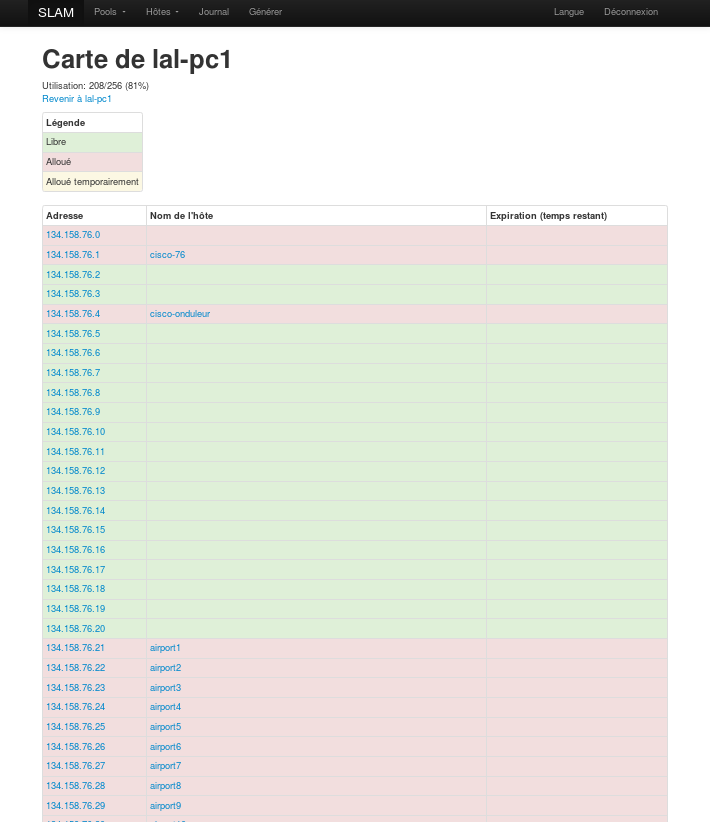
\includegraphics[scale=0.45]{img/web3}
	\caption{Carte d’un Pool d’adresses}
	\label{fig:web3}
\end{figure}

Suite à la création de cette carte, une nouvelle information a été ajoutée aux
adresses~: la possibilité de déclarer une allocation temporaire avec une durée
attachée. Cela est uniquement à caractère informatif, mais, du coup, ce type
d’information est répercuté sur la page de carte des Pools avec une couleur
différente et la durée associée est affichée afin de suivre ce type
d’allocations.\\

À la suite d’une réunion de suivi, il a été décider de refaire une partie du
cœur du logiciel afin de donner une place centrale aux catégories de machine et
d’adresse. L’idée était d’avoir un comportement qui ne varie pas en fonction
des pools dans lequel un hôte a une adresse, mais en fonction de sa catégorie.
Cette modification était nécessaire pour résoudre un certain nombre de
problèmes et permettre de nouvelles fonctionnalités. La génération automatique
des noms de machine dérivés des adresses IP pouvait ainsi être gérée à ce
niveau, de même que la façon dont sont gérés les alias dans les fichiers de
configuration générés qui diffèrent selon que l’hôte est un serveur ou un poste
de travail.
\label{sec:newmodel}

Cependant cette décision a été prise trois semaines avant la fin du stage, et,
après avoir débuté les premières modifications au cœur du logiciel, il a été
décidé que le nombre de composants impactés était trop grand et demanderait la
réécriture d’une partie imposante des deux interfaces, des tests et de la
documentation. Cette modification a donc été abandonnée, mais reste versionnée
dans le gestionnaire de version du projet et a été documentée en détail afin
qu’une éventuelle continuation soit possible à l’avenir par une autre
personne.\\

Les deux dernières semaines du stage ont été dédiées à la migration définitive
des données existantes et au perfectionnement du logiciel. Pour la migration,
il a suffi de modifier le Makefile existant côté DNS et le fichier de
configuration principal du serveur DHCP pour ne plus prendre en compte les
anciens fichiers et utiliser uniquement les nouveaux fichiers générés par SLAM.
Cependant, plusieurs problèmes ont retardé la migration de quelques jours.

Le premier problème rencontré est la gestion des champs DNS de type \verb+MX+
spécifiques à certains hôtes. Il existait ainsi cinq machines disposant de
serveurs de messagerie électronique différents de ceux par défaut et le
logiciel SLAM et les scripts de migration n’ont pas d’option prévue afin de
générer ce cas particulier. Une méthode a donc été créée en utilisant une
propriété (expliqué en section \ref{sec:property}, page \pageref{sec:property})
avec un nom particulier dont la valeur sera insérée telle quelle dans le
fichier de configuration généré. Cette solution est peu élégante, mais c’était
celle qui paraissait la plus rapide et celle qui ne modifiait pas de parties
critiques du logiciel pour les adapter aux besoins spécifiques du laboratoire,
ce qui permet de garder la réutilisabilité du logiciel désirée depuis le début
du développement.

Un autre problème était la gestion des dépendances du Makefile pour la
génération des fichiers de configuration DNS ainsi que le script TCL qui
s’occupait de la transformation du format spécifique au LAL vers le format
utilisé par le serveur DNS. Pour le Makefile, il a suffi de rafraîchir la
date de dernière modification des fichiers pour qu’il rafraîchisse tous les
fichiers utilisés. Le problème était que le script TCL allait chercher les
anciens fichiers de configuration afin de générer les enregistrements inverses
DNS des zones. Il a donc suffi de supprimer ces fichiers, en prenant soin de
les sauvegarder avant, pour que le script fonctionne bien à partir des bons
fichiers. Il manquait également plusieurs informations qui ne sont pas créées
par le script, mais ont été écrites statiquement et laissées telles quelles par
le script de génération. Il a alors suffi de reporter ces informations dans le
nouveau fichier pour obtenir un résultat correct, fidèle aux fichiers de
configuration initiaux. De plus, cette migration a permis de se débarrasser
d’un certain nombre de lignes de configuration devenues obsolètes.

Une page a enfin été ajoutée à l’interface graphique pour pouvoir exécuter le
script qui s’occupe de transférer les fichiers de configuration sur les bons
serveurs et de relancer les différents services. Il n’a pas été trop difficile
d’exécuter le script depuis l’interface Web, en récupérant correctement les
sorties standard et d’erreur. Il y avait cependant des problèmes de droit pour
l’écriture des fichiers de configuration, mais cela a été réglé en ajustant les
droits de ces fichiers de configuration.\\

L’outil a fini par être installé sur une machine virtuelle dédiée où seront
également installés d’autres outils d’administration. Des difficultés ont été
rencontrées pour déployer l’interface Web derrière un serveur \emph{Apache2},
le module permettant d’interagir avec une application Python, \verb+mod_wsgi+,
ayant un problème connu. Le souci a été réglé en recompilant le module dans
sa version la plus récente.

Enfin, quelques dernières modifications ont été apportées à l’interface Web
pour améliorer son utilisabilité. Des boutons ont ainsi été ajoutés aux
différentes listes d’objets afin de changer le tri effectué sur ces listes. Il
est ainsi possible de trier une liste d’hôtes par nom, par adresse IP, par
adresse MAC\dots De plus, de gros ralentissements pouvaient être ressentis au
moment de charger la page listant l’intégralité des hôtes du réseau du
laboratoire à cause de leur très grand nombre. Une nouvelle page a donc été
créée afin de pouvoir rechercher dans cette liste d’hôtes. La possibilité
d’allouer une nouvelle adresse à un hôte a été ajoutée, permettant ainsi, après
avoir désalloué une adresse d’un hôte, de lui en réattribuer une nouvelle
directement depuis l’interface Web. Enfin, la possibilité de supprimer les
anciennes entrées de journal a été ajoutée à l’interface Web, afin d’éviter que
le journal ne devienne trop gros et donc trop long à charger.

\subsection{Activités auxiliaires}

Le stagiaire a été invité à participer à plusieurs activités complémentaires,
qui n’étaient pas directement liées à son activité, mais se rapportaient à la
vie du laboratoire, ou du service et qui lui ont permis de mieux découvrir la
vie du laboratoire et du service.\\

Un événement récurrent est la tenue hebdomadaire des réunions
d’exploitation auxquelles était invité le stagiaire. Ces réunions étaient
organisées entre les membres de l’équipe exploitation et le chef de service et
avaient pour but de présenter les dernières avancées de chacun au cours de la
semaine précédente et de donner les orientations et priorités pour la semaine à
venir. Ces réunions étaient également l’occasion de discuter de sujets en
rapport avec le système d’information du laboratoire. Un des derniers sujets à
avoir été discuté concernait par exemple une directive du CNRS qui exigeait que
tous les postes de travail du laboratoire chiffrent systématiquement les
données sauvegardées des utilisateurs. La question était de savoir comment
faire pour les trois plateformes principales, Windows, Linux et Mac~OS et
comment faire en sorte de chiffrer les postes du parc existant.

L’outil développé au cours de ce stage a eu l’occasion d’être montré sous sa
forme ligne de commande afin de présenter le logiciel à l’équipe et de
recueillir des remarques sur cette interface. L’interface Web devait aussi être
présentée au cours d’une réunion, mais n’a pas pu l’être, par manque de temps.
Elle a donc été présentée aux personnes intéressées a posteriori.\\

Du côté de l’équipe développement, des réunions, les \og~Dev Loops~\fg{},
sont organisées une fois par mois et consistent en une présentation des
travaux effectués ou des technologies, concepts ou méthodologies découvertes
récemment et susceptibles d’intéresser les autres développeurs. Le stagiaire
n’a pu assister qu’à une de ces réunions où étaient présentés les sujets
suivants~:

\begin{itemize}
	\item \emph{Hadoop} par Julius \textsc{Hrivnac}, présentation de cette base
	de données \emph{NoSQL} et son utilisation par le projet Atlas,
	\item \emph{LLVM} par Sebastien \textsc{Binet}, présentation de ce
	framework pour compilateurs et des utilisations qui peuvent en être faites,
	\item \emph{Utiliser StratusLab au LAL pour un développeur} par Laurent
	\textsc{Garnier}, retour d’expérience sur la création d’une VM avec cet
	outil de gestion Cloud pour un projet,
	\item \emph{Boost} par François-David \textsc{Collin}, présentation de
	cette bibliothèque C++ et son déploiement,
	\item \emph{OpenID} par Oleg \textsc{Lodygensky}. mise en place de cette
	solution permettant de déléguer l’authentification à d’autres entités.
\end{itemize}
~\\

Concernant les réunions à l’échelle du laboratoire, deux assemblées générales
auront été organisées au cours du stage, pour présenter les sujets généraux qui
touchent l’ensemble des équipes et menées par le directeur du laboratoire,
Achille \textsc{Stocchi}. Il y a par exemple été expliqué le plan de rénovation
P2IO, expliqué en section \ref{sec:context}, page \pageref{sec:context}, ou
bien la liste des découvertes scientifiques de l’année 2012, la liste des
thèses du laboratoire ou la liste des personnes ayant quitté ou rejoint le
laboratoire. Pendant cette réunion, il est intéressant de noter que n’importe
qui pouvait poser des questions directement au directeur.\\

Enfin, des journées de conférences étaient organisées avec différentes
thématiques. Le service informatique a par exemple organisé la journée
\emph{Cloud}, dont le but était de présenter différentes solutions de Clouds,
dont celle développée au sein du laboratoire ainsi que leurs différentes
applications dans le monde de la recherche. Elle était suivie, le lendemain,
par un atelier sur l’outil de virtualisation \emph{StratusLab}, développé au
laboratoire pour apprendre à tous ceux que ça intéresse à lancer leurs machines
virtuelles.

\newpage

\section{Revue du travail accompli}

Le logiciel SLAM a été correctement achevé pendant la période couverte par le
stage et il a été déployé et mis en production sur le système informatique du
LAL. La totalité des machines sont maintenant gérées avec ce logiciel en ce qui
concerne le DNS et le DHCP et il n'y a plus d'autre méthode possible pour les gérer.
Plusieurs membres de l’équipe utilisent déjà ce
logiciel pour la gestion des machines. Une documentation est fournie avec le
logiciel pour expliquer son installation, son utilisation, son fonctionnement
interne et de potentiels axes de développement si une autre personne devait
continuer le développement, le tout en anglais et sans détails spécifiques au
laboratoire afin de prévoir son éventuelle distribution grand public future.
Une documentation en français est, par ailleurs, fournie et couvre toutes les
spécificités du logiciel pour son utilisation dans le cadre du service. Enfin,
de nombreux tests ont été écrits afin de vérifier le bon fonctionnement d’à peu
près tous les aspects du logiciel.\\

Il est cependant dommage que le changement de modèle détaillé en section
\ref{sec:newmodel}, page \pageref{sec:newmodel} n’ai pas pu être suffisamment
développé. Cela aurait pu aboutir à des solutions plus élégantes pour certaines
fonctionnalités spécifiques au LAL. De plus, même si l’interface en ligne de
commande a été améliorée afin d’être plus intuitive, elle demeure assez
inconfortable à utiliser et mériterait un plus grand soin. L’interface
Web est par contre tout à fait utilisable sans difficulté.

\begin{center}
\begin{figure}[hbt]
	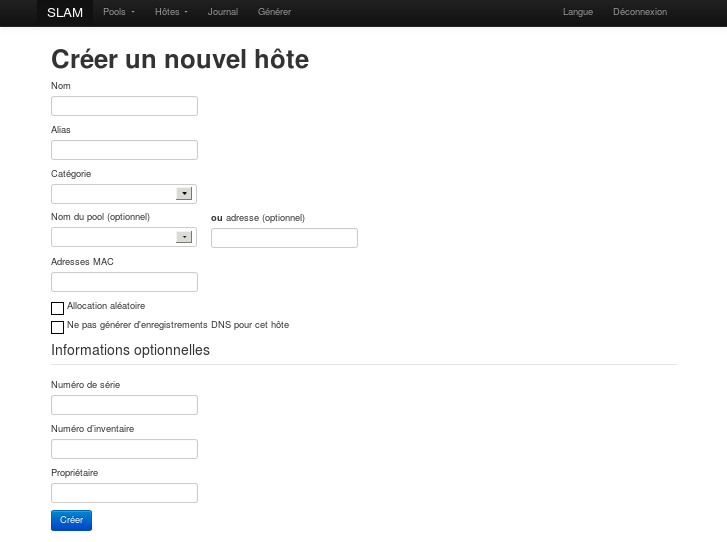
\includegraphics[scale=0.45]{img/web5.png}
	\caption{Exemple de page Web du logiciel~: ajout d’hôte}
	\label{fig:web5}
\end{figure}
\end{center}

La documentation générale en anglais couvre tous les aspects du logiciel, mais
manque peut être de détails sur certaines parties délicates. De même, si toutes
les fonctions et modules contiennent une courte description de leur rôle,
certaines parties délicates du code manquent peut être de commentaires. Une
page de documentation a aussi été écrite sur l’interface TRAC dédiée au
service informatique et une autre sur la page TRAC dédié au projet SLAM afin
d’expliquer la procédure d’installation et l’utilisation qui peut en être
faite, en français cette fois, et contenant tous les détails spécifiques au
laboratoire.

Concernant les tests, ils couvrent bien toutes les parties de SLAM, mis à part
la génération du HTML par Django, ce qu’on peut considérer comme anecdotique,
car il est doublé par une génération en \emph{Json} qui est, elle, testée
soigneusement, ainsi qu’à plusieurs niveaux~: unitaires et fonctionnels. Ils
auraient cependant pu être beaucoup plus fournis afin de tester des cas plus
pathologiques et auraient permis d’éviter certains bugs découverts à
posteriori.\\

Comme décrit dans la documentation finale, voici les pistes
d’amélioration qui pourraient être apportées au logiciel~:

\begin{itemize}
	\item le nouveau modèle basé sur les catégories d’hôtes et d’adresse comme
	expliqué précédemment, tous les détails de cette transformation ainsi que
	son état actuel sont expliqués dans la documentation,
	\item simplification de l’interface en ligne de commande, la piste
	d’utiliser un meilleur module afin de récupérer les arguments de la ligne
	de commande a été envisagée,
	\item générer le fichier de zone au format DNS directement plutôt que de
	passer par un format intermédiaire. En effet SLAM permet tout à fait de
	générer ce type de format, en plus du format personnalisé utilisé par le
	laboratoire. Il serait possible de migrer cette partie entièrement vers
	SLAM, en prenant soin de bien intégrer les données statiques qui ne peuvent
	pas être gérées par SLAM grâce à l’option d’inclusion d’en-têtes avant les
	données générées par exemple,
	\item interaction avec le serveur DHCP, probablement en analysant les
	journaux générés par celui-ci, afin de mettre à jour la date de dernière
	utilisation d’une adresse, ce qui est déjà prévu grâce à une option de la
	ligne de commande. Il ne reste donc plus qu’à lire et analyser les journaux
	générés par le fichier DHCP et fournir un moyen de lister les adresses qui
	ne sont plus utilisées depuis un certain temps.
\end{itemize}
~\\

Enfin, il est dommage que le manque de temps ait empêché l’élaboration d’un
paquet Python et sa distribution libre afin de faire profiter du logiciel tous
ceux qui pourraient en avoir besoin.

\chapter{Conclusion}

Le stage a été l’occasion de développer un logiciel de gestion automatique des
adresses IP, avant tout pour les besoins du laboratoire dans lequel il se
déroulait, mais également pour une éventuelle distribution libre afin de
pouvoir être réutilisé par d’autres entités.

La gestion des adresses se traduit ainsi par la possibilité de mettre en
relation des hôtes et des adresses sélectionnées dans des collections
d’adresses appelées Pools. Deux interfaces, l’une en ligne de commande afin
d’être facilement scriptable et accessible de n’importe où et l’autre sous
forme de site Web pour proposer une plus grande facilité de gestion, doivent
permettre l’ajout, modification et suppression des différents types d’objets
définis précédemment~: pools, hôtes et adresses et de gérer toutes les
interactions qu’il peut y avoir entre ces objets. Le logiciel doit finalement
permettre la génération automatique de fichiers de configuration pour les
différents services réseau impactés par son fonctionnement à savoir le serveur
DNS et le serveur DHCP. Ce logiciel devait également être accompagné d’une
documentation conséquente et de tests afin de pouvoir être convenablement
maintenu une fois le stage terminé.\\

Le développement du logiciel a donc eu lieu pendant toute la durée du stage en
suivant une méthodologie AGILE, ce qui implique des réunions de suivi
régulières pour régler les différentes questions ou incertitudes qui pourraient
apparaître au cours du développement. Grâce aux choix de technologies bien
documentées et plutôt populaires, aucun problème majeur n’a été rencontré
pendant le développement du logiciel, les quelques petits problèmes ayant été
résolus par de simples recherches ou expérimentations. La migration des données
existantes a commencé à être envisagée et planifiée progressivement à partir
du milieu du stage environ et en prenant soin de tester toutes les étapes dans
un environnement de test avant de le déployer en production.\\

Ce stage a été l’occasion de découvrir le fonctionnement de l’équipe
exploitation d’une grosse structure et d’acquérir de nouvelles connaissances
grâce à l’utilisation d’un très grand nombre de technologies intervenant à tous
les niveaux du développement d’un logiciel ainsi que l’expérience apportée par
la migration et le déploiement d’un service central au fonctionnement des
postes informatiques du laboratoire.

Finalement, le cahier des charges a été respecté~: le logiciel a été
correctement déployé et est utilisé par les membres de l’équipe du service
informatique pour la gestion des machines du laboratoire. Les anciennes
données ont correctement été migrées et sont donc gérées par SLAM et la
configuration des serveurs DNS et DHCP est maintenant faite par SLAM.

\appendix

\part*{Annexes}

\section*{Exemple de fichier de documentation~: Installation de la VM SLAM}

Procédure d’installation de la VM SLAM spécifique au LAL.

\subsection*{Prérequis}

\subsubsection{Packages à installer}

\begin{itemize}
	\item \verb+git+
	\item \verb+python2+ (≥ 2.6)
	\item \verb+django+ (≥ 1.4)
	\item \verb+python-argparse+
	\item \verb+python-ldap+
	\item \verb+MySQL-python+
	\item \verb+httpd+
	\item \verb+mod_wsgi+ (≥ 3.3)
	\item \verb+gettext+
\end{itemize}
~\\

Pour la doc et les tests (facultatifs pour le fonctionnement réel de SLAM)~:

\begin{itemize}
	\item \verb+python-nose+
	\item \verb+python-sphinx+
\end{itemize}

\subsubsection{Modules à installer hors du gestionnaire de paquets}

\begin{itemize}
	\item \verb+django-auth-ldap+
	\begin{itemize}
		\item installer le paquet \verb+python-pip+
		\item \verb+python-pip install django-auth-ldap+
	\end{itemize}
	\item \verb+mod_wsgi+ obligatoirement en version 3.3 (http://code.google.com/p/modwsgi/)
	\begin{itemize}
		\item installer les paquets \verb+httpd-devel+ \verb+python-devel+ \verb+make+ \verb+gcc+
		\item \verb+./configure && make && make install+
	\end{itemize}
\end{itemize}

\subsubsection{Autre}

\begin{itemize}
	\item Le NFS \verb+/mgt+ doit être monté,
	\item l’utilisateur apache doit avoir les droits d’écriture vers les fichiers et dossiers~:
	\begin{itemize}
		\item \verb+/mgt/named/src/lal.slam+
		\item \verb+/mgt/dhcp/conf/dhcpd.conf.slam-net+
		\item \verb+/mgt/dhcp/conf/dhcpd.conf.slam-pc1+
		\item \verb+/mgt/dhcp/conf/dhcpd.conf.slam-pc2+
		\item \verb+/mgt/named/src/backup/+
		\item \verb+/mgt/dhcp/conf/backup/+
	\end{itemize}
\end{itemize}

\subsection*{Installation de SLAM}

\begin{itemize}
	\item \verb+cd /srv+
	\item \verb+git clone http://git.lal.in2p3.fr/projects/slam.git+
	\item \verb+mkdir /etc/slam+
	\item contenu de \verb+/etc/slam/users+~:
\begin{lstlisting}
root
apache
\end{lstlisting}
	\item contenu de \verb+/etc/slam/configuration.py+ avec le \verb+PASSWORD+ dans \verb+DATABASES+ et le \verb+AUTH_LDAP_BIND_PASSWORD+ à compléter~:
\begin{lstlisting}[language=python]
DEBUG = False
ADMINS = (
    # ('Your Name', 'your_email@example.com'),
)

DATABASES = {
    'default': {
        'ENGINE': 'django.db.backends.mysql',
        'NAME': 'SI_SLAM',
        'USER': '',
        'PASSWORD': '',
        'HOST': '',
        'PORT': '', # not used
    }
}
TIME_ZONE = 'Europe/Paris'
LANGUAGE_CODE = 'fr-FR'
SECRET_KEY = r"""random"""
ROOT_DIR = "/srv/slam"
RELOAD_SCRIPT = "/srv/slam/scripts/slam_reload"

# LDAP configuration
import ldap
from django_auth_ldap.config import LDAPSearch
AUTH_LDAP_SERVER_URI = ""
AUTH_LDAP_BIND_DN = ""
AUTH_LDAP_BIND_PASSWORD = ""
AUTH_LDAP_USER_SEARCH = LDAPSearch("",
    ldap.SCOPE_SUBTREE, "(samaccountname=%(user)s)")
AUTHENTICATION_BACKENDS = (
    'django_auth_ldap.backend.LDAPBackend',
    'django.contrib.auth.backends.ModelBackend',
\end{lstlisting}
	\item contenu de \verb+/etc/httpd/conf.d/slam_wsgi.conf+~:
\begin{lstlisting}
WSGIScriptAlias / /srv/slam/src/webinterface/wsgi.py
WSGIPythonPath /srv/slam/src
#WSGIRestrictEmbedded On

<Directory /srv/slam/src/webinterface>
<Files wsgi.py>
Order deny,allow
Allow from all
</Files>
</Directory>

Alias /assets /srv/slam/assets

<Directory /srv/slam/assets>
Order deny,allow
Allow from all
</Directory>
\end{lstlisting}
	\item \verb+cd /srv/slam/src/webinterface && ../manage.py compilemessages+
	\item \verb+/etc/init.d/httpd restart+
	\item Pour pouvoir exécuter le script \verb+slam_reload+ et relancer les serveurs DNS et DHCP, l’utilisateur apache doit pouvoir se ssh root sur asa et as3 sans password (→ générer une clé RSA sans passphrase et mettre la clé publique sur le Tru64 et la clé privé dans \verb+/var/www/.ssh+).
\end{itemize}

\subsection*{Si Apache sert des 403 forbidden}

SELinux peut causer des problèmes, il faut essayer de désactiver le mode enforced (\verb+setenforce 0+).

% the following was generated by SPHINX

\section*{Exemple de documentation principale en anglais~: architecture interne}
\label{internal:internals}\label{internal::doc}

\subsection*{Technologies}
\label{internal_general:technologies}\label{internal_general::doc}
This is a summary of the technologies SLAM uses and what they are used for:
\begin{itemize}
\item {} 
SLAM, the actual tool
\begin{itemize}
\item {} 
\textbf{python} (2.6) as the main programming language

\item {} 
\textbf{Django} (\emph{python-django}): framework used as Web interface and as
an ORM for the application

\item {} 
\textbf{SQLite} as the database backend, can be changed by users by only
changing one configuration variable

\end{itemize}

\item {} 
SLAM's versioning system
\begin{itemize}
\item {} 
\textbf{Git}: distributed versioning system

\end{itemize}

\item {} 
SLAM's installation
\begin{itemize}
\item {} 
custom \textbf{shell} script: automatic configuration of the project

\item {} 
\textbf{python} script provided by Django: initialize the database, start
the Web server…

\end{itemize}

\item {} 
SLAM's testing and integration, used for code-style, unit, functional
testing
\begin{itemize}
\item {} 
\textbf{pylint}: very customizable coding-style and programming mistakes
checker

\item {} 
\textbf{NOSE} (\emph{python-nose}): simple and complete test framework for
Python applications

\item {} 
\textbf{NOSE's coverage plugin} (\emph{nose-cov}): used to get a complete and
precise report on the test-suite code coverage

\item {} 
\textbf{Jenkins}: continuous integration software that poll the repository
and automatically launch the full sytle and test-suite each day or
for any change in the repository

\end{itemize}

\item {} 
SLAM's documentation and project management
\begin{itemize}
\item {} 
\textbf{SPHINX} (\emph{python-sphinx}): generate the documentation in multiple
formats (HTML, PDF, epub, texinfo…) from \emph{reStructuredText} files

\item {} 
\textbf{Trac}: the Wiki and the bug tracker are the main tools we use

\end{itemize}

\end{itemize}


\subsection*{Global Architecture}
\label{internal_general:global-architecture}

\subsubsection{Core}
\label{internal_general:core}
The core of the project is composed of models: Host, Pool, Address, Property
that are the structures used by Django to represent data in the database; the
address ranges and collections: Ip4Range for IPv4, Ip6Range for IPv6 and
AddressSet for arbitrary addresses; and generators that output configuration
file for a specific software or service.

Most of the core processing happens in the address ranges and in the \emph{Pool}
class. Address ranges store a collection of address and \emph{Pool} keeps track of
the status of the address of one of these collection (allocated or available).

Properties can be added to a \emph{Host} or a \emph{Pool} and can be used to add any
information of type (key: value).


\subsubsection{Interfaces}
\label{internal_general:interfaces}
Two interfaces are provided by default : CLI and Web with Django. They interact
directly with the SLAM Django application through the \textbf{slam.interface}
module. This module provides several helper function to perform various usual
task. New interfaces should use these functions as much as possible but can
very well interact directly with the SLAM Django application.


\paragraph{REST and Web interfaces}
\label{internal_general:rest-and-web-interfaces}
It was chosen to merge these two interfaces because a lot of code would have
been duplicated between these two interfaces if they were split. Furthermore,
thanks to Django's template system and its REST middleware, the distinction is
really no that strong. It also allow to only test the REST interface with the
JSON output and consider the Web interface is tested as well because the
treatments are exactly the same and parsing the JSON output is far easier than
HTML.

For user input, the problem was that HTML does not allow the generation of
query with PUT and DELETE method which are required to provide a sane REST
interface (it was added to the HTML5 specification at some point but has been
removed since). However a really simple Django middleware can be used to
transparently make the conversion between POST request with hidden fields and
HTTP methods which allow us to receive only proper REST query without any
effort.

For output, a simple in-url setting (\emph{format}) allow the user to specify that
he expect a specific output format such as \emph{json}. This is implemented really
easily thanks to Django's template system and the only difference between the
HTML and JSON format is the template used.


\paragraph{Interface Translation}
\label{internal_general:interface-translation}
We chose to only translate the Web interface. This is done easily with the
internationalization module of Django which generate automatically \emph{.po} files
for easy translation.


\subsubsection{Generators}
\label{internal_general:generators}
Generators inherit from \emph{Confg} in \textbf{slam.generator} and can overwrite
\emph{gen\_header}, \emph{gen\_footer} and \emph{generate} to customize the behavior of the
generator. For example, the \emph{Bind} generator uses \emph{gen\_header} to parse the
\emph{SOA} record and increment it. They can also declare their format of comment
that will be used to generate the SLAM headers in the generated configuration
file.


\subsubsection{Tests}
\label{internal_general:tests}
Tests are stored in their own files in the \textbf{/test} directory, regrouped by
tested python modules. They are executed on an independant database. Tests that
need to compare output use \emph{StringIO} and test that need to provide an input
stream uses a simple pipe.

\end{document}
